  
\documentclass[titlepage]{article}
\usepackage[utf8]{inputenc}
\usepackage{amsmath}
\usepackage{tcolorbox}
\usepackage{amssymb}
\usepackage{amsthm}
\usepackage{empheq}
\usepackage{hyperref}
\usepackage{listings}
\usepackage{xcolor}
\usepackage{float}
\usepackage{xparse}
\usepackage{mathtools}
\DeclarePairedDelimiter{\ceil}{\lceil}{\rceil}
\usepackage[
top    = 2.50cm,
bottom = 2.50cm,
left   = 2.75cm,
right  = 2.75cm]{geometry}
\usepackage{fancyhdr}
\pagestyle{fancy}
\lhead{AICC 2}
\rhead{EPFL/Alp Ozen}

\newtheorem{remark}{Remark}[section]
\newtheorem{theorem}{Theorem}[section]
\newtheorem{lemma}[theorem]{Lemma}
\newtheorem{prop}{[Proposition]}
\newtheorem{definition}{Definition}
\newtheorem{question}{Question}


\newcommand{\interior}[1]{%
  {\kern0pt#1}^{\mathrm{o}}%
}
\newcommand{\Rn}{\mathbb{R}^n}
\newcommand{\Rm}{\mathbb{R}^m}
\newcommand{\R}{\mathbb{R}}

\title{\textbf{AICC 2 - Bixio Rimoldi}}
\author{Alp Ozen}
\date{Spring 2019}
\newtheorem{example}{Example}[section]
\newtheorem{axiom}{Axiom}
\newtheorem{cor}{Corollary}

\begin{document}

\maketitle
\clearpage

\section{Week 2}

\subsection{Entropy}
We begin by defining \textbf{entropy} as Shannon put it:

\begin{definition}\textbf{Entropy}

Note that this definition assumes base $2$ aka. binary.
$$ H(s) = - \sum_{s \in A} p(s)\log_{2}p(s) \ \text{A being our alpahabet aka. sample space}$$
and thus an equivalent definition is:
$$ H(s) = E[-\log_{2}p(s)]$$
And similarly, Shannon defines information as:
$$-\log_{2}p(s)$$
\end{definition}

For a random distribution we get:

\begin{example}
$$\forall x \in A \ p(x) = \frac{1}{|A|}, \ -\log_{2}p(s) = \log_{2}|A|$$
Hence the entropy function $H(s) = E[\log_{2}|A|]} = \underbrace{\log_{2}|A|}_{\text{do the algebra}}$
\end{example}

And now we present the \textbf{information theory inequality}

\begin{definition}\textbf{IT inequality}
$$ \log_{b}r \leq (r-1)\log_{b}(e)$$
\end{definition}

\begin{proof}
Given that $$\ln(r) \leq (r-1)$$ and that $$ ln(r) = \frac{\log_{b}(r)}{\log_{b}(e)}$$ we are done.
\end{proof}

And now we present the Entropy bound theorem:
\begin{theorem}
$$S \in A \ 0 \leq H(S) \leq \log|A|$$ 
\end{theorem}

\begin{proof}
We only show the RHS as the LHS is more or less trivial. 
Our goal is to show:

\begin{align*}
    \text{need to reach} H(s) - \log|A| \leq 0 \\
    E[-\log p(s)] - \log |A|\\
    = E[\log \frac{1}{p(s)|A|}]\\
    = \sum_{s\in A}p(s)(\log \frac{1}{p(s)|A|})\\
    \leq \underbrace{log(e)\sum[\frac{1}{|A|} - p(s)]}_{\text{using IT ineq.}} = 0
\end{align*}
\end{proof}
\subsection{Source coding}
A code is said to have a prefix if:
\begin{definition}\textbf{Prefix of a code}
\\

For some sequence of characters $a_{1}a_{2}\ldots a_{n}$ and $b_{1}b_{2}\ldots b_{m}$ with $n \leq m$ we have $a_{1}a_{2}\ldots a_{n} =  b_{1}b_{2}\ldots b_{n}$
\end{definition}

A \textbf{prefix free code} also known as \textbf{instantaneouss code} is one that has no prefixes. And now we come to the important \textbf{Kraft-McMillan} result:

\begin{theorem}
If a $D-ary$ code is uniquely decodable, then it satisfies:

$$ D^{-l_{1}} + \ldots + D^{-l_{m}} \leq 1 $$
\textcolor{red}{Note that there are non-instantaneous codes that stil satisfy this inequality. By the same token, by the contrapositive, we have that if a code does not satisfy the inequality, then there exists no prefix-free version of it.}
\end{theorem}

We now define the \textbf{average codeword length}

\begin{definition}\textbf{average codeword length}
$$ L(S,R) = \sum_{s \in A} p_{S}(s)L(R(s)) \ \text{where $L$ represents length}$$
\end{definition}

Given this definition, another important result is:

\begin{theorem} \textbf{Lower bound and Upper bound for average optimal codeword length}
$$H_{d}(S) \leq L(S,R) \leq H_{d}(S) + 1$$
\end{theorem}

This result becomes a useful tool once we realize the similarity in the definitions as below:

\begin{align*}
    H(S) = - \sum p(s)\log p(s)\\
    L(S,R) = \sum p(s)L(R(s))
\end{align*}

Given this, \textit{Shannon - Fano} realized that we may define a code of length $\ceil*{\log_{D} p(s)}$
This satisfies the Kraft inequality hence we now have a method of obtaining uniquely decodable code. 
\\

But as it turns out, Huffman was the first to actually find out how one finds an optimal code. We list our alphabet with probability in increasing order. Then, if say we are working in base 2, we simply continuously combine the smallest probabilities and build our branches from them. Hence, as below, we have that a Huffman code isn't always unique:

\begin{figure}[H]
    \centering
    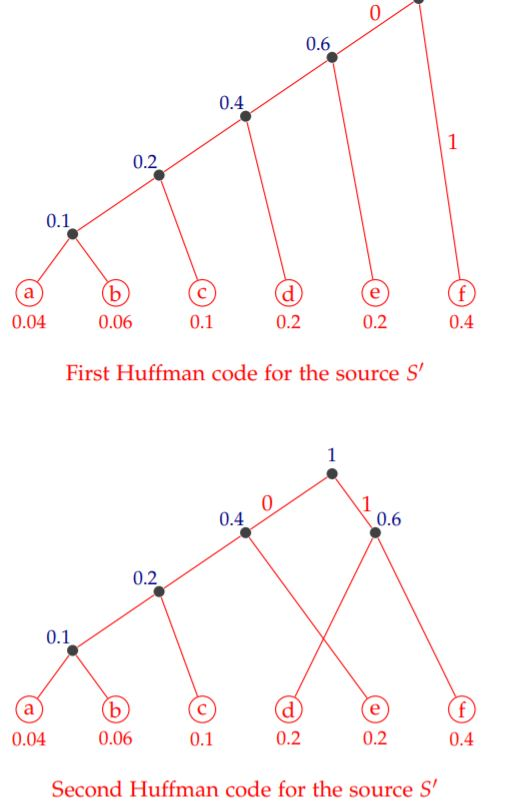
\includegraphics[scale = 0.3]{src/huff.JPG}
    \caption{Huffman codes}
    \label{fig:my_label}
\end{figure}

\section{Week 3}
We now define conditional entropy(the intuition for this being, we want to mesure uncertainty given knowledge of something else) as follows:

\begin{definition}
$$H(X|Y) := - \sum p(x|y)\log p(x|y)$$
\end{definition}

And the law of \textbf{total probability}

\begin{theorem}
Imagine we take a sample space with some subset $A$ and cut it into 3 disjoint units $B_{i}$. Now we may describe the set $A$ as $A = (B_{1} \cap A) \cup (B_{2} \cap A) \cup (B_{3} \cap A)$ This is equivalent to now saying:

$$p(A) = p(B_{1} \cap A) + p(B_{2} \cap A) + p(B_{3} \cap A) $$
Which in terms of conditional probability is $$p(A) = p(A|B_{1})p(B_{1}) + p(A|B_{2})p(B_{2}) + p(A|B_{3})p(B_{3})$$
\end{theorem}

And another useful theorem is:

\begin{theorem}
$$H(s_{1},s_{2},\ldots,s_{n}) \leq H(s_{1}) + H(s_{2}) + \ldots + H(s_{n})$$
with equality iff the $s_{i}$ are independent. 
\end{theorem}

A similar result now is the chain rule of conditional entropy.
\begin{theorem}\textbf{Conditional entropy chain rule}
$$H(S_{1},S_{2},\ldots,S_{n}) = H(S_{1}) + H(S_{2}|S_{1}) + \ldots + H(S_{n}|S_{1},\ldots,S_{n-1})$$
\end{theorem}

To clarify the notation used above, when we write $P_{X_{1}}, \ldots, X_{n}(x_{1},\ldots, x_{n})$ we interpret each comma as an intersection$\cap$

And we now introduce what it means for a source to be \textbf{regular}

\begin{definition}\textbf{Regular source}
\\
A source is regular if
\begin{align*}
    H(S) := \lim_{n\to\infty} H(S_{n})\\
    H^{*}(S) := \lim_{n \to \infty} H(S_{n}|S_{1},S_{2},\ldots,S_{n-1})
\end{align*}

exist and are finite. 
\end{definition}

Now it should be intuitively obvious that conditioning would reduce entropy. Lets prove it.

\begin{theorem}
$$H(X|Y) \leq H(X)$$
\end{theorem}

\begin{proof}
\begin{align*}
    E(\log\frac{1}{p(X|Y)}) + E(\log p(X))\\
    = E(\log\frac{p(X)}{p(X|Y)})\\
    = E(\log\frac{p(X)p(Y)}{p(X|Y)p(Y)})\\
    \leq (\frac{p(X)p(Y)}{p(X\cap Y) - 1}\log(e)
    \leq 0
\end{align*}
\end{proof}

\section{Week 4}

We begin by making an important distinction in the definition of conditional entropy.

\begin{definition}\textbf{Conditional entropy given $Y=y$}
\\
We define this as:
$$H(X|Y=y) = - \sum_{x \in (\cdot | y)} P(x|y)\log P(x|y)$$
\end{definition}

Given this definition, the more general definition of conditional entropy is:

\begin{definition}
$$H(X|Y) = - \sum P(y)H(X|Y=y) $$
\end{definition}

And we now introduce a \textbf{stationary source}

\begin{definition}\textbf{Stationary source}
\\
A source is stationary if $\forall n,k$ the blocks $S_{1}, \ldots, S_{n}$ and $S_{n+1}, \ldots, S_{k}$ have the same statistic that is:
\begin{align*}
    P_{s_{1}} = P_{s_{i}}
\end{align*}

\end{definition}


\begin{theorem}
All stationary sources are regular. 
\end{theorem}

And now we come to another intuitive result:
\begin{theorem}
$$H^{*}(S) = \lim_{N\to \infty}\frac{H(S^{n})}{n}$$
\end{theorem}

The intuition for this result is that the entropy rate is inversely proportional to how much information we have. That is the more variables we know, the more we reduce entropy. 

We now consider an instructive example
\begin{example}
Suppose we are given two machines $M_{1}$ and $M_{2}$ that produce 3 bits. $M_{1}$ produces any number between 0 and 7 with equal chance and $M_{2}$ produces a number in range 0 to 3 with equal chance. We ask then, what is the probability distribution of the sequence $s_{1}\ldots s_{n}$

Well noticing that this is equal to finding 

$$ P(S_{1}\ldots S_{n})=P(S_{1}\ldots S_{n}|S_{0})P(S_{0}) = P(S_{1}\ldots S_{n}|S_{0})P(S_{0} = M_{1}) + P(S_{1}\ldots S_{n}|S_{0})P(S_{0} = M_{2})$$

We obtain:
$$P(S_{1}\ldots S_{n}) = \[   \left\{
\begin{array}{ll}
     \frac{1}{8^{n}}\frac{1}{2} + \frac{1}{4^{n}}\frac{1}{2} \text{if} s_{1}\ldots s_{n} \in \{0,\ldots,3\}^{n}\\
     \frac{1}{8^{n}}\frac{1}{2}
\end{array} 
\right. \]$$
\end{example}

\section{Week 5}
This week, we introduce cryptography. 
We begin by listing the most common attack methods.

\begin{itemize}
    \item \textbf{Chosen-plaintext attack}: The attacker is able to obtain a ciphertext for any arbitrary plaintext. Thus to obtain the key, one might encode every single letter. 
    \item \textbf{Known-plaintext attack}: Attacker has access to both ciphertext and plaintext.
    \item \textbf{Ciphertext-only attack}: Attacker has access to a set of ciphertexts. A possible attack method is to use a frequency analysis. 
\end{itemize}

We now introduce the vigenere cipher.
\begin{definition}\textbf{Vigenere's cipher}
Vigenere cipher makes use of the Caesar cipher. Suppose we are given a 7 letter plaintext. The sender chooses another keyword of 7 letters. This we call the key. Then encryption is done using the lookup table below.

\begin{figure}[H]
    \centering
    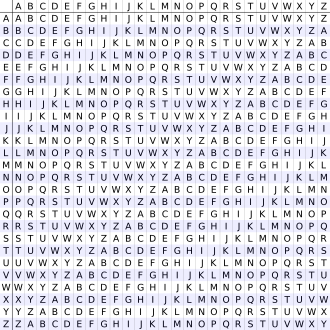
\includegraphics[scale = 0.6]{src/vigenere.png}
    \caption{Lookup table}
    \label{fig:my_label}
\end{figure}

As an example suppose our plaintext is "hello", an example key is "abcde". Thus the encrypted word would become "hffos"
\end{definition}

Now we introduce a very strong type of secrecy. 

\begin{definition}\textbf{Perfect secrecy}
A cryptosystem has perfect secrecy if the plaintext and ciphertext are statistically independent. 
\end{definition}

Given this perfect secrecy implies:
\begin{theorem}
H(T) \leq H(K)
\end{theorem}

And now we present an instructive example on how one would try to crack vigenere given we have the ciphertext and a portion of the plaintext.

\clearpage

\begin{example}\textbf{Cracking Vigenere}
\begin{figure}[H]
    \centering
    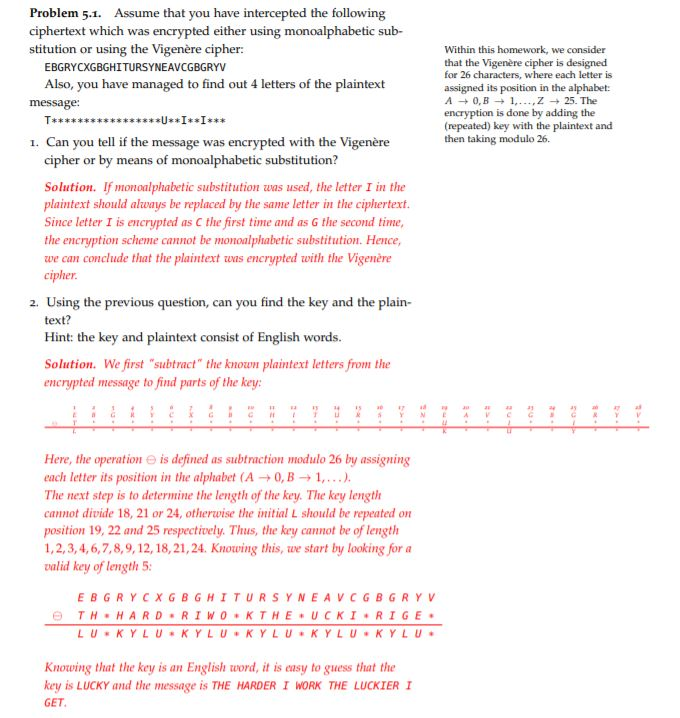
\includegraphics{src/vig.JPG}

    \label{fig:my_label}
\end{figure}
\end{example}

We know present a method used to verify the correctness of data sent.
\begin{example}
Suppose we want to send an IBAN number over the net. It is possible that for some reason, during transmission, two digits of the credit card get flipped. We need a system to verify the correctness of information sent. Here's how we proceed:
\begin{itemize}
    \item concatenate 00 to the end of the IBAN number.
    \item mod out by 97, fix this as $a$.
    \item now our key $k$ is found as $98-a=k$
    \item concatenate $k$ to the end of the IBAN number removing the 00 and now send it to the recipient
    \item receiver mods out by 97, if result is congruent to 1, success.
\end{itemize}

Here is why this works:
Given $x \equiv a \mod{97}$
\begin{align*}
    x^{\prime} \equiv x + (98 - a) \mod{97}\\
    x^{\prime} \equiv x + 98 - x \mod{97}\\
    x^{\prime} \equiv 98 \mod{97} \equiv 1 \mod{97}\\
\end{align*}

Yet another proof is to show the following implication:
$$100n_{97} - 100\Tilde{n}_{97} \equiv 0_{97} \implies a=b \text{where a,b are changed digits}$$

Now our above equality simplifies to:

$$10^{k+1}a+10^{k}b - 10^{k+1}b - 10^{k}a = 10^{k}(9a-9b)$$
Now since all expressions in the above equations have an inverse as we are in base 97, we get:
$$ (a-b)_{97} \equiv 0_{97}$$
which is only the case if $a=b$
\end{example}

A neat modulo trick is presented below.

\begin{theorem}
For some number $a = d_{n}\ldots d_{1}$ in base 10 we have that:
$$a \bmod{11} = \sum_{i}^{k}10^{i}d_{i} \bmod{11} = \underbrace{\sum_{i}^{k}-1^{i}d_{i}}_{10\equiv-1\bmod{11}} \bmod{11}$$
\end{theorem}

\section{Week 6}

We present some definitions and theorems which we later use to define certain structures in $\mathbb{R}$.

\begin{definition}\textbf{Ring}
A ring is a triple $(R,\alpha,\mu)$ such that the following hold:
\\

$R,\alpha$ known as the 'addition' on $R$ is an abelian group 
\\

$R, \mu$ is both associative and right-left distributive over addition
\\

If it is also the case that $R/{e_{\alpha}}$ is an abelian group, our ring is called a \textit{commutative ring with unity}

\end{definition}
\\

\begin{theorem}
The inverse of an element under any binary relation is unique.
\end{theorem}

\begin{proof}
Let $ab = e$ and also $ac=e$. Then $abb=acb$ which simplifies to $eb=ec=b=c$
\end{proof}

\begin{theorem}
Within $\mathbb{Z} / m\mathbb{Z}$ the following theorems are equivalent:
\\

$\forall a \in \mathbb{Z}, \exists a^{-1}$
\\

$f:\forall a \in \mathbb{Z} \to \forall a \in \mathbb{Z}$ is a bijection
\\

$ax=b$ has a unique solution 

\end{theorem}

\begin{theorem}
Some $[a]_{m}$ has a multiplicative inverse iff $gcd(a,m)=1$
\end{theorem}


Given the above, something that easily follows is:

\begin{theorem}
If $p$ is prime, then all $a \in \mathbb{Z}/p\mathbb{Z}$ have a multiplicative inverse 
\end{theorem}

\begin{remark}\textbf{Useful facts about the gcd}
$$gcd(a,b) = gcd(b,a-kb)=gcd(\pm a, \pm b)$$
\end{remark}

We now present the Euclidian algorithm used to find $gcd(a,b)$ in pseudocode and explain why it works.


\begin{lstlisting}
if(a<b) return:
gcd(b,a);
else if(b=0) return:
a;
else return:
gcd(b,a\% b);
\end{lstlisting}

\begin{theorem}\textbf{Bezout's theorem}
$$gcd(a,b) = au + bv \ a,b \in \mathbb{Z}$$
\end{theorem}

We now ask given the above theorem, how we may find the $u$ and $v$. Well let's take an example:
\begin{example}
Find the $u,v$ for $gcd(56,15)$.
By normal Euclidian algorithm, it turns out that $gcd(56,15) = 1$ Our steps in finding this are:
\begin{align*}
    56 = 15(3) + 11\\
    15 = 11(1) + 4\\
    11 = 4(2) + 3\\
    4 = 3(1) + 1\\
    3 = 1(3) + 0
\end{align*}

Now notice how we from the above already have:
$$56 - 15(3) = 11 \ 4 - 3(1)=1$$
Hence all that's left to do now is make $4 - 3(1)=1$ top and work our way down.
\begin{align*}
    4 - 3(1) = 1\\
    4 -  11 + 4(2)\\
    4(3) - 11\\
    (15 - 11(1))3 - 11\\
    15(3) - 11(4)\\
    15(3) - (56-15(3))4\\
    (-4)56 + (12)15 
\end{align*}

\end{example}

\begin{lemma}
$$gcd(a,m) = 1 \iff \ \exists u,v \ 1 = au + mv$$
\end{lemma}




We now explore some notation relating to modular classes:
\begin{itemize}
    \item $[a]_{m} :=$ congruence class $\bmod{m}$
    \item $\mathbb{Z} / m\mathbb{Z} :=$ all congruence classes $\bmod{m}$
    \item The structure $<\mathbb{R} / m\mathbb{Z}, + , \cdot>$ is an abelian ring 
    \item By $\mathbb{Z} / m\mathbb{Z}^{*}$ we denote the set where an inverse exists. 
\end{itemize}

\begin{definition}\textbf{Totient function}
 $\phi (x): \mathbb{Z} \to \mathbb{N}$ computes the number of integers that are relatively prime to $x$.
\end{definition}

\begin{lemma}
When $p$ is prime, $\phi(p) = p-1$
\end{lemma}

\begin{remark}
The cardinality of $\mathbb{Z} / m\mathbb{Z}^{*}$ is $\phi(m)$
\end{remark}

\begin{remark}
$$\phi (p^{k}) = p^{k} - p^{k-1}$$ for some prime $p$
\end{remark}

Yet another super useful result that appears in RSA encryption is the following:
\begin{remark}
Let $p$ and $q$ be prime numbers, we ask what is $\phi (pq)$
$$\phi (pq) = pq - (p + q -1) = (p-1)(q-1) = \phi (p) \phi (q)$$
which follows from the fact that the numbers relatively prime to $pq$ are:
$$ \[   \left\{
\begin{array}{ll}
     p,2p,\ldots, qp\\
     q,2q,\ldots,(p-1)q
\end{array} 
\right. \]$$
\end{remark}

Finally we define perhaps one of the most fundemental mathematical structures, that is an isomorphism.

\begin{definition}\textbf{Isomorpishm}
\\

 Let $(H_{1},\cdot_{1})$ and $(H_{2},\cdot_{2})$ be two structures. An isomorphism $\phi$ from $H_{1}$ to $H_{2}$ is bijection such that:
 $$\forall a,b \in H_{1} \ \phi(a\cdot_{1} b) = \phi(a)\cdot_{2} \phi(b)$$
\end{definition}

Now isomorphisms are useful because we know that if $(H_{1},\star})$ is an abelian group and there exists an isomorphism from to $(H_{2},\star_{2}})$, then so is $$(H_{2},\star_{2}})$ an abelian group. 
\\

Now perhaps a mind blowing isomorphism is between the structures $([0, + \infty] \cdot)$ and $(\mathbb{R},+)$ The isomorphism between the two is simply any mapping $f(x) = \log_{b}(x)$

Now we present a theorem about finite groups:

\begin{theorem}
Let $G$ be a finite group. Then $\forall a \in G$, $\exists k \in \mathbb{Z_{+}}$ such that $a^{k} = e$
\end{theorem}

\begin{proof}
Now since $G$ is a finite group, we have that for some $i < j$ , $a^{i} = a^{j}$. Now
$a^{-i}a^{i} = a^{-i}a^{j} = a^{j-i} = a^{k}$
\end{proof}

And now a theorem about the order of elements in a group. 

\begin{theorem}
Two sets are isomorphic iff. they have the same order set. 
\end{theorem}

And now a grand result from the early developments of group theory.

\begin{theorem}\textbf{Lagrange's theorem}
Let $G$ be a finite abelian group of cardinality $n$. Then the order of each elements of $G$ divides $n$. 
\end{theorem}

\begin{proof}
Let $H \leqslant G$. Now the cosets of $H$ form a partition of $G$ as the coset is an equivalence relation. Also note that $H$ as a subgroup is of the form $\{a,a^{2},\ldots,a^{k}\}$ where $k$ is the order of $a$. Hence we have that $|H| = k$. Now we have that $G$ is a partition of equivalence classes all of size $k$ that is to say:

$$ n = kq \ \text{q being number of equivalence classes}$$
\end{proof}

We now present a corollary of Lagrange's theorem that will prove useful when studying RSA.

\begin{cor}\textbf{Euler's theorem}
\\

Let $m > 1$. $\forall a \in (\mathbb{Z} / mZ^{*})$ we have:
 $$a^{\phi(m)} = [1]_{m}$$
\end{cor}

Now a result following Euler's theorem is that if we apply the same reasoning to some $(\mathbb{Z} / pZ^{*})$ where $p$ is prime then $\phi(p) = p-1$ hence $a^{p-1} = e$ and $a^p = a$

\begin{theorem}\textbf{Chinese remainder theorem}
Let $m_{1},m_{2}$ be co-prime integers. We define a mapping $\phi: Z/m_{1}m_{2}^{*} \to  Z/m_{1} \cross Z/m_{2} $ Then it is the case the the mapping is a bijection and an isomoprhism with respect to $+$ and $\cdot$, where $\phi:(a)_{m_{1}m_{2}} \to (a)_{m_{1}}(a)_{m_{2}}$
\end{theorem}

Let us now expand on our understanding of groups. 

\begin{definition}\textbf{Cyclic group}
A group $G$ where $\exists g \in G$ such that $\forall h \in G, \exists i \in \mathbb{Z} \ h = g^{i}$ is called a cyclic group. 
\end{definition}

It turns out that all cyclic groups of the same order are isomorphic. As a quick sketch of proof, consider that we define a map as $\psi(a^{i})=b^{i}$. Then simply observe that 

$$\psi(ab) = \psi(g^{i}g^{j}) = \psi(g^{i+j})=h^{i+j}=\psi(a)\psi(b)$$

A concrete example of an isomorphism between groups is the map from $(\mathbb{Z}/m\mathbb{Z},+) \to (G,\star)$ where $G$ is cyclic. We define it as $[i]_{n} \to b^{i}$ $n$ being the order of $G$


\section{Week 7}
We now consider what's called the discrete exponent problem. Suppose we have a finite group $G,\star$ of size $N$ with generator $g$. We are asked to find the $\alpha$ such that $h = g^{\alpha}$. Doing this the bruteforce way would be to construct all elements $g^{i}$ with $i\leq \alpha$ at the cost of $\alpha - 1$ which is $O(n)$. But we can do better. We pick some $k$ and compute all $g^{k}$. We also then compute $bg^{-i}$. Now we suppose some common element such that $g^{n} \equiv hg^{-mi} \bmod{n}$ Then we have that $a^{mi+n} = h$ which solves the problem. This will take us $O(\frac{N}{B})$ steps.
\\

We are now ready to present the RSA encryption scheme.
\begin{definition}\textbf{RSA scheme}
Let $K_{pr} = \{d,m\}$ be the private key and $K_{p} = \{e,m\}$ our public key. Upon Bob wanting to send Alice a message, Alice sends $K_{p}$ to Bob which Bob uses the encrpyt his message and send the ciphertext back to Alice. But before, to come up with $e,m$ Alice must pick to large primes $p$ and $q$ and $m$ must a multiple of $p-1$ and $q-1$. We may do this either by taking $lcm(p-1,q-1)$ or by taking $\phi(pq)$. Now here is how we derive the rest of the scheme:
We start of with Euler's theorem which states for $m,n$ are coprime:
$$m^{\phi(n)} \equiv 1 \bmod{n}$$
Now what suits are need is a relation of the form:
$$m^{k\phi(n) + 1} \equiv m \bmod{n}$$
Hence we have that:
$$ed = k\phi(n)+1$$
Now the reason finding a $d$ that satisfies this is equivalent to finding an integer(guaranteed to exist through Bezout because we selected $e$ coprime to $\phi(n)$) that satisfies:
$$d = \frac{k\phi(n)+1}{e}$$
But for someone who doesn't know our $p$ and $q$ this is extremely hard since they must factor $n$ into two primes to calculate $\phi(n)$. 
\end{definition}


\section{Week 8 onwards}
We now move our focus to the physical transmission of data through channels. We have two types of channels: \textbf{error channels} and \textbf{erasure channels}. Erasures can occur for instance due to destructive interference or some networking error. Now let's introduce some terminology. A \textbf{code block} is some $C \subseteq A^{n}$. The \textbf{code rate} is defined as $\frac{k}{n}$ with $k = \log_{|A|}{|C|}$. The question at this stage is, what is the most efficient way to choose an optimal code correcting encoding. We define the \textbf{Hamming distance} between two source codes as:
$$d(x,y) = |\{i \in \{1,\ldots,n\} \ x_{i} \not = y_{i} \}|$$
Hence the minimal distance is that between some $x,y \in C$ such that $d(x,y)$ is minimum. To develop intuition for this, a minimum Hamming distance implies the maximum number of errors we can detect. If for instance some encoding has a minimum distance of $4$, then we can detect an error of size 3 but not of 5. Thus the larger the distance, the better. Now two theorems.

\begin{theorem}
An encoding is able to correct an erasure if an only if its weight is $p < d_{min}$
\end{theorem}

\begin{theorem}
An encoding is able to correct an error if and only if its weight is $p < \frac{d_{min}}{2}$
\end{theorem}

We now ask how many searches do we need in general to determine $d_{min}$ for some encoding. Taking the brute-force approach we have that for the first code we do $m-1$ for the second $m-2$... checks which means our search is $O(\frac{m^{2}-m}{2})$. 
\\

Another question to be asked is, for our code block what properties would we like? First of all, $d_{min}$ should be as large as possible to allow for maximum error correction. Similarly, $n(\text{length of code block})$ should be as small as possible for minimal data storage. Finally, $|C|$ should be as large as possible because then each code block will be carrying maximal information. In answer to this, we have the Singleton bound theorem which states:

\begin{theorem}
For some code block $C$ of length $n$ and $k = \log_{|A|}{|C|}$ we have:
$$d_{min}(C) - 1 \leq n- k$$
\end{theorem}
\\

At this stage to further our discussion of how we determine $d_{min}$ with a complexity better than a quadratic one we must introduce some algebraic structures. 

\begin{definition} \textbf{Field}
\\
A field is a triplet $(K, + , \cdot)$ with the following property:
$$ (K, +) \ \text{and} \ (K/\{0\}, \cdot) \ \text{are abelian groups}$$
Some examples of non-finite fields are:
$$((\mathbb{R}, \mathbb{Q}, \mathbb{C}), +, \cdot)$$
\end{definition}

\begin{definition} \textbf{Vector space}
\\
A non-empty set $V$ is a vector space over a field $F$ if:
\begin{enumerate}
    \item There exists a binary operation $+$ where $\forall a,b \in V$, $a+b \in V$
    \item There is a mixed operation called scalar multiplication $(\cdot)$ where $\forall c \in F$ and $\forall v \in V$ we have $c\cdot v \in V$
    \item and the below hold:
    \begin{itemize}
        \item $(V,+)$ is a commutative group 
        \item associativity: $(ab)v = a(bv)$
        \item identity: $1v = v$
        \item scalar multiplication is right,left distributive over addition 
    \end{itemize}
\end{enumerate}
\end{definition}

Our first theorem about fields states the following:

\begin{theorem}
The order of $1(\text{multiplicative identity})$ with respect to $+$ is a prime number. This specific order is known as the characteristic of a field.
\end{theorem}

\begin{proof}
Suppose that the order of $1$ is $m$ and $m$ is not prime letting $m = ab$. Then we have:

$$\underbrace{1 + \hdots + 1}_{m} = 0$$
$$\underbrace{(1 + \hdots + 1)}_{a} \underbrace{(1 + \hdots + 1)}_{b} = 0$$
Now we have that either $a$ or $b$ must be $0$. But this then implies that $m = 0$ and $m$ is supposed to be a smallest non-zero integer. Hence we have a contradiction. 

Now, in analogue to groups, two fields are said to be the 'same' if there is an isomorphism between two fields. Namely a bijective map that respects both of $(+,\cdot)$. 
\end{proof}

\begin{theorem}
\begin{enumerate}
    \item The cardinality of a finite field is an integer power of its characteristic.
    \item All finite fields of the same cardinality are isomorphic.  
    \item For every prime $p$ and positive integer $m$, there exists a finite field of cardinality $p^{m}$
\end{enumerate}
\end{theorem}

Thus we have that for each $p,m$ there exists exactly one field of cardinality $p^{m}$. Otherwise said, all finite fields of cardinality $p^{m}$ are isomorphic to each other. To introduce some notation, a field of cardinality  $p^{m}$ is denoted $\mathbb{F}_{p^{m}}$ or $\mathbb{GF}(p^{m})$

\begin{example}
$$F_{2} = (\mathbb{Z}/2\mathbb{Z}, +, \cdot)$$
$$F_{3} = (\mathbb{Z}/3\mathbb{Z}, +, \cdot)$$
\end{example}

But we quickly realize that we can't further state that $F_{4} = (\mathbb{Z}/4\mathbb{Z}, +, \cdot)$ since $2$ would not have a multiplicative inverse. So let's construct $F_{4}$, it looks like the below: 

$$\vbox{\tabskip0.5em\offinterlineskip
    \halign{\strut$#$\hfil\ \tabskip1em\vrule&&$#$\hfil\cr
    +   & 0   & 1   & a & b     \cr
    \noalign{\hrule}\vrule height 12pt width 0pt
    0   & 0   & 1   & a & b    \cr
    1   & 1   & 0&  b  & a    \cr
    a & a & b   & 0  & 1    \cr
    b   & b   & a   & 1   & 0   
  
}}$$

The way we constructed the above is as follows:
\begin{itemize}
    \item We know the characteristic is $2$ so along the right diagonal all entries are 0. 
\end{itemize}
\\

Similarly, we can also construct the multiplication table which looks as follows:
 $$\vbox{\tabskip0.5em\offinterlineskip
    \halign{\strut$#$\hfil\ \tabskip1em\vrule&&$#$\hfil\cr
    \cdot   & 0   & 1   & a & b     \cr
    \noalign{\hrule}\vrule height 12pt width 0pt
    0   & 0   & 0   & 0 & 0    \cr
    1   & 0   & 1&  a  & b    \cr
    a & 0 & a   & b  & 1    \cr
    b   & 0   & b   & 1   & a   
  
}}$$
\\

It is now time to use our understanding of vector spaces and fields to build so-called \textit{linear codes}.

\begin{definition}\textbf{Linear code}
A code $C \subseteq \mathbb{F}^{n}$ is linear $C$ is a subspace of $\mathbb{F}^{n}$. Given this definition of $C$ as a subspace, we add the note that the cardinality of $C$ is precisely $|F|^{k}$ for the reason that $k$ is our dimension hence we have $k$ many choices to make out of $|F|$ many possibilities.
\end{definition}


\begin{figure}[H]
    \centering
    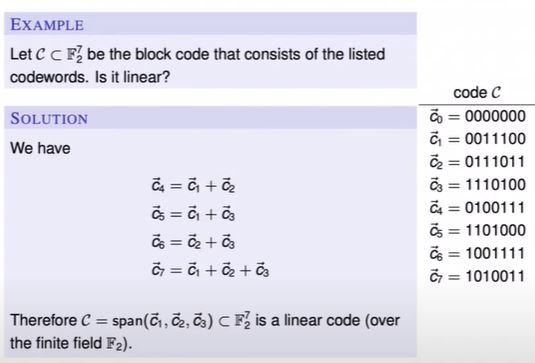
\includegraphics{src/lin1.JPG}
    \caption{Example of a linear code}
\end{figure}

\begin{theorem}
If $V$ is an $n$ dimensional vector space over some finite field $F$, then $V$ is finite and $card(V) = card(K)^{n}$
\end{theorem}

Using the above theorem, we have a means to check if a code $C$ is a linear code over $F_{p^{m}}$. We simply verify that $card(C) \not = p^{mk}$. 
\\

We now present a theorem about minimal distance. Defining \textbf{Hamming weight} denoted $\omega(\vec{x}) = d(\vec{0},\vec{x})$ we have that:

$$d_{min}(C) = \min_{\vec{x} \in C,  \vec{x} \not = \vec{0}}}{\omega{(\vec{x})}}$$
\\

We now come to discuss \textit{generator matrices}. A generator matrix has as it rows the basis vectors for some code $C$. Clearly bases are not unique hence we can have more than one generator matrix, but precisely how many? To see this, let $(\vec{c_{1}}, \ldots, \vec{c_{k}})$ be a basis. How many choices of $\vec{c_{1}}$ are there? Well given that $|F| = q$ we have $q^{k}-1$ choices where we subtract a one to account for the zero vector. Then for $\vec{c_{2}}$ we have $q^{k}-q$ many choices. This time we subtract $q$ because there are $q$ many scalar multiples of $\vec{c_{1}}$ that we must exclude. Hence the total number of generator matrices for a code $C$ turns out to be: $(q^{k}-1)(q^{k}-q)\ldots(q^{k}-q^{k-1})$.
\\
We say that a generator matrix is in \textit{systematic form} if it is of form:
$$G_{s} = [\underbrace{I_{k}}_{kxk}, \underbrace{P}_{kxn-k}]$$
Another way to view a systematic generator matrix is to say that it is in \textit{reduced echelon form}. The advantage of a systematic generator matrix is that our encoding mapping is as follows:
$$\vec{u} \in \mathbb{F}^{k} \to \vec{c} = (\vec{u}, \vec{u}P)$$ which means that the first $k$ entries of the output vector correspond exactly to our information bits hence inverting the encoding function(which a decoder does) is as simple as reading the first $k$ entries of the codeword. 

\section{Useful links}
Amazing YouTube playlist: \hyperlink{ https://www.youtube.com/playlist?list=PLE125425EC837021F}{YT Information Theory playlist}



\end{document} 
